% --------------------------------------------------------------
% This is all preamble stuff that you don't have to worry about.
% Head down to where it says "Start here"
% --------------------------------------------------------------
 
\documentclass[12pt]{article}
 
\usepackage[margin=1in]{geometry} 
\usepackage{amsmath,amsthm,amssymb}
\usepackage[margin=1in]{geometry} 
\usepackage{amsmath,amsthm,amssymb}
%\usepackage[spanish]{babel} %Castellanización
\usepackage[T1]{fontenc} %escribe lo del teclado
\usepackage[utf8]{inputenc} %Reconoce algunos símbolos
\usepackage{lmodern} %optimiza algunas fuentes
\usepackage{graphicx}
\graphicspath{ {images/} }
\usepackage{hyperref} % Uso de links
 
\newcommand{\N}{\mathbb{N}}
\newcommand{\Z}{\mathbb{Z}}
 
\usepackage{listings}
\usepackage{xcolor}

\definecolor{codegreen}{rgb}{0,0.6,0}
\definecolor{codegray}{rgb}{0.5,0.5,0.5}
\definecolor{codepurple}{rgb}{0.58,0,0.82}
\definecolor{backcolour}{rgb}{0.95,0.95,0.92}

\lstdefinestyle{mystyle}{
    backgroundcolor=\color{backcolour},   
    commentstyle=\color{codegreen},
    keywordstyle=\color{magenta},
    numberstyle=\tiny\color{codegray},
    stringstyle=\color{codepurple},
    basicstyle=\ttfamily\footnotesize,
    breakatwhitespace=false,         
    breaklines=true,                 
    captionpos=b,                    
    keepspaces=true,                 
    numbers=left,                    
    numbersep=5pt,                  
    showspaces=false,                
    showstringspaces=false,
    showtabs=false,                  
    tabsize=2
}

\lstset{style=mystyle}


 
\begin{document}
 
% --------------------------------------------------------------
%                         Start here
% --------------------------------------------------------------
 
\title{Turorial 7: Strings}
\date{}
\author{APS 105: Computer Fundamentals\\ %replace with your name
Winter2020}

\maketitle
This week we cover strings, as they are very important in all modern programming languages. In the following examples, we first focus on how strings are processed with the help of character by character operations. Then, we will try some useful functions to tackle these things. 
\section{Character by character operations(a)}
In this part, we will learn how to initialize a string in different ways and change the specific parameter within the given string.
\begin{lstlisting}[language=C, caption=Solution 1]
void Q1()
{
    printf("Q1:\n");
    //Approach 1
	const int LENGTH = 5; 
    //Declaring and initializing a string as a character array
    char str[LENGTH + 1];
    str[0] = 'H';
    str[1] = 'e';
    str[2] = 'l';
    str[3] = 'l';
    str[4] = 'o';
    str[5] = '\0';
    
    printf("Approach 1: str = %s\n", str);
    
    //Approach 2
    char s[] = "Hello";
    // The length of the string could be ignored.
    // However, if you declare a string without enough space, for example "char s[4] = "Hello";"
    // A compile-time warning and run-time error would occur
    
    printf("Approach 2: s = %s\n", s);
    
    //Approach 3
    char *p = "Hello";
    // Declaring and initializing a string as a character pointer
    printf("Approach 3: p = %s\n", p);
    
    
    //Now try to change the characters in the string s
    printf("\n");
    s[1] = 'E';
    printf("s = %s\n", s);
    // But you cannot change s to point to another string. 
    // For example, "s = "HELLO;" is wrong!!!
    // A compile-time erro, which is "array type is not assignable", will occur
    
    // You can switch the pointer variable p to another string
    p = "HELLO";
    printf("p = %s\n", p);
    // You cannot change characters in the string pointed to by p
    // For example, "p[1] = 'E';" is wrong!
    // It may cuase a segmentation fault or bus error (on Mac OS X)
    
    
    // Compare the pointer values to see where these strings are
    printf("\nThe pointer variable of s: %p\n", s);
    printf("The pointer variable of p: %p\n\n", p);
    
    // Now let p point to s, so that we can safely change the characters
    p = s;
    printf("p = %s\n", p);
    
    p[2] = 'L';
    printf("p = %s\n", p);
    
    }
\end{lstlisting}
The output is shown in fig. \ref{output1}.

\begin{figure}[h]
%\centering
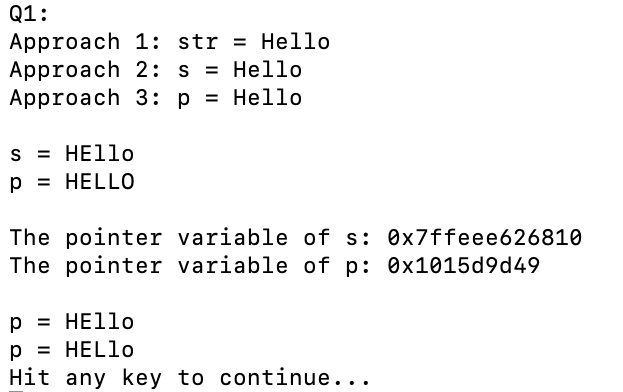
\includegraphics[scale=0.85]{Images/output1.png} 
\caption{Output 1}
\label{output1}
\end{figure}


\section{Character by character operations(b)}
In this part, we will try to compute the number of words in the given sentence by applying character to character operations we learnt above.

\begin{lstlisting}[language=C, caption=Solution 2]
void Q2()
{
    printf("Q2:\n");
    char s[] = "This is a given sentence.";
    int numberOfSpaces = 0;
    
    for(int i = 0; s[i] != '\0'; i++)
    {
        if (s[i] == ' ')
            numberOfSpaces++;
    }
    
    printf("The sentence is:\n");
    puts(s);// We can use puts() to print a string
    printf("The number of words in the given sentence is %d\n",numberOfSpaces + 1);
    }
\end{lstlisting}
The output is shown in fig.\ref{output2}.
\begin{figure}[h]
%\centering
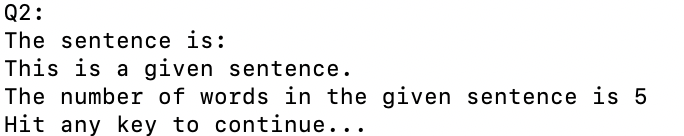
\includegraphics[scale=0.85]{Images/output2.png} 
\caption{Output 2}
\label{output2}
\end{figure}

\section{Basic string functions(a)}

Currently, many useful functions were predefined for you, meaning that you could simply use those functions in your own program, without worrying about how the strings are processed within the functions. So, please just try to use them. In this problem, we would look for the index of the specific character in the given string. 

(Hints: The $strchr()$ function finds the first occurrence of a character in a string. The character $c$ can be the null character ($\setminus0$); the ending null character of string is included in the search.) 

\begin{lstlisting}[language=C, caption=Solution 3]
void Q3()
{
    // strchr: Looking for a specific character in a given string
    printf("\nQ3:\n");
    char s[] = "This is a given string";
    char a;
    printf("What are you looking for?\n");
    scanf("%c",&a);
    printf("Looking for the character '%c' in \"%s\"...\n", a, s);
    
    char *p = strchr(s, 's');
    
    while (p != NULL) 
    {
        printf("Found at %ld\n",p - s + 1);
        p = strchr(p + 1, 's');
    }
}
\end{lstlisting}

The output is shown in fig. \ref{output3}.


\begin{figure}[h]
%\centering
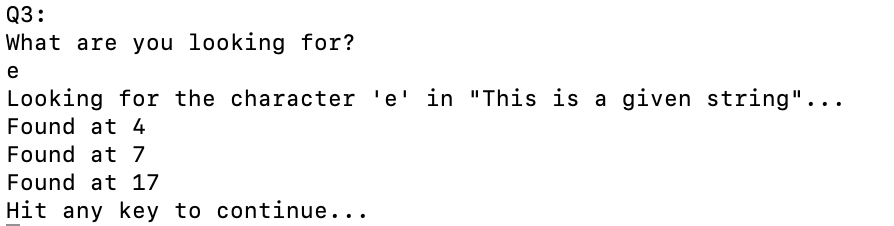
\includegraphics[scale=0.85]{Images/output3.png} 
\caption{Output 3}
\label{output3}
\end{figure}
\section{Basic string function(b)}
Let's explore more! 
\begin{lstlisting}[language=C, caption= Solution 4]
void Q4()
{
   printf("Q4:\n");
   char s1[99];
   char s2[99];
   
   printf("\nPlease enter a string:\n");
   gets(s1);//Instead of "scanf"
   printf("The string you entered is:\n");
   puts(s1);//Instead of "printf"
   
   printf("Length of the string is: %lu\n", strlen(s1));
   //strlen(string) could compute the length of the string
 
   printf("\nPlease enter another string:\n");
   gets(s2);
   
   if (strcmp(s1, s2) ==0) // strcmp(string1, string2) could compare these two strings 
     {
        printf("str1 and str2 are equal.\n");
     }else
      {
         printf("str1 and str2 are different.\n");
      }
   
   printf("\nLet's concatenate these two strings:\n");
   strcat(s1,s2); // Concatenate string1 and string2.
   printf("Output string after concatenation: %s\n", s1);
   
   printf("\nLet's copy the string str1 into string str2:\n");
   strcpy(s2,s1);//copy string1 into string2,including the end character '\0'
   printf("Str2 is: %s\n", s2);
   
    }
\end{lstlisting}{}
The output is shown in fig. \ref{output4}

\begin{figure}[h]
%\centering
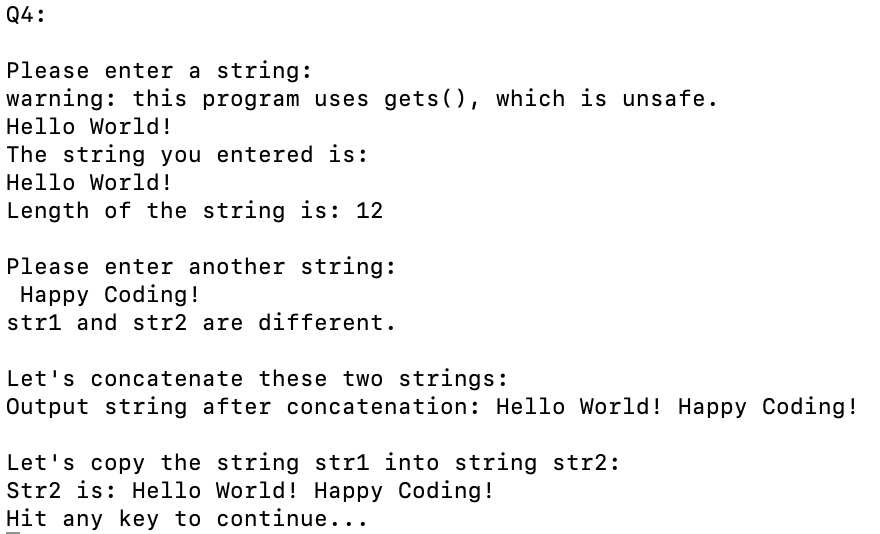
\includegraphics[scale=0.85]{Images/output4.png} 
\caption{Output 4}
\label{output4}
\end{figure}

% --------------------------------------------------------------
%     You don't have to mess with anything below this line.
% --------------------------------------------------------------
 
\end{document}